\section{Cahier des charges}
Cette partie présente le cahier des charges du périphériques.
Elle intègre les quelques points fournis par le sujet auquel s'ajoutent les contraintes imaginées par les étudiants.
\hl{...}
\subsection{Objectif du circuit}
Le contrôleur d'interruptions a l pour rôle d'informer le processeur sur l’occurrence d'une interruption valide.
Il fournira alors l’adresse de la prochaine instruction à exécuter.

\subsection{Fonctionnalitées attendues}
Les fonctions de service du circuit sont :
\begin{enumerate}
    \item Masquer et démasquer chaque interruption individuellement
    \item Contenir le vecteur d'exception
    \item Etablir le niveau de priorité des interruptions
    \item Ne fournir au \gls{CPU} que les interruptions valides
    \item Prendre en compte les priorités dans la génération des demandes au \gls{CPU}
\end{enumerate}
\subsection{Utilisation du circuit}
	
Il s'agit ici de donner l'utilisation du circuit en présentant le schéma de câblage du contrôleur d'interruptions ainsi que la définition des signaux logiques d'entrées et sorties.
L'\gls{IP} à concevoir s'interface avec le bus de données, le bus d'adresses ainsi qu'un ensemble de signaux de temporisation et de contrôle.
Il est possible de retrouver des signaux de temporisation comme le nWAIT et des signaux de contrôle comme le nRST ou le RnW.
Leur rôle est présenté table (\ref{tab:sens_role_signaux}).
	
\begin{figure}[H]
	\centering
	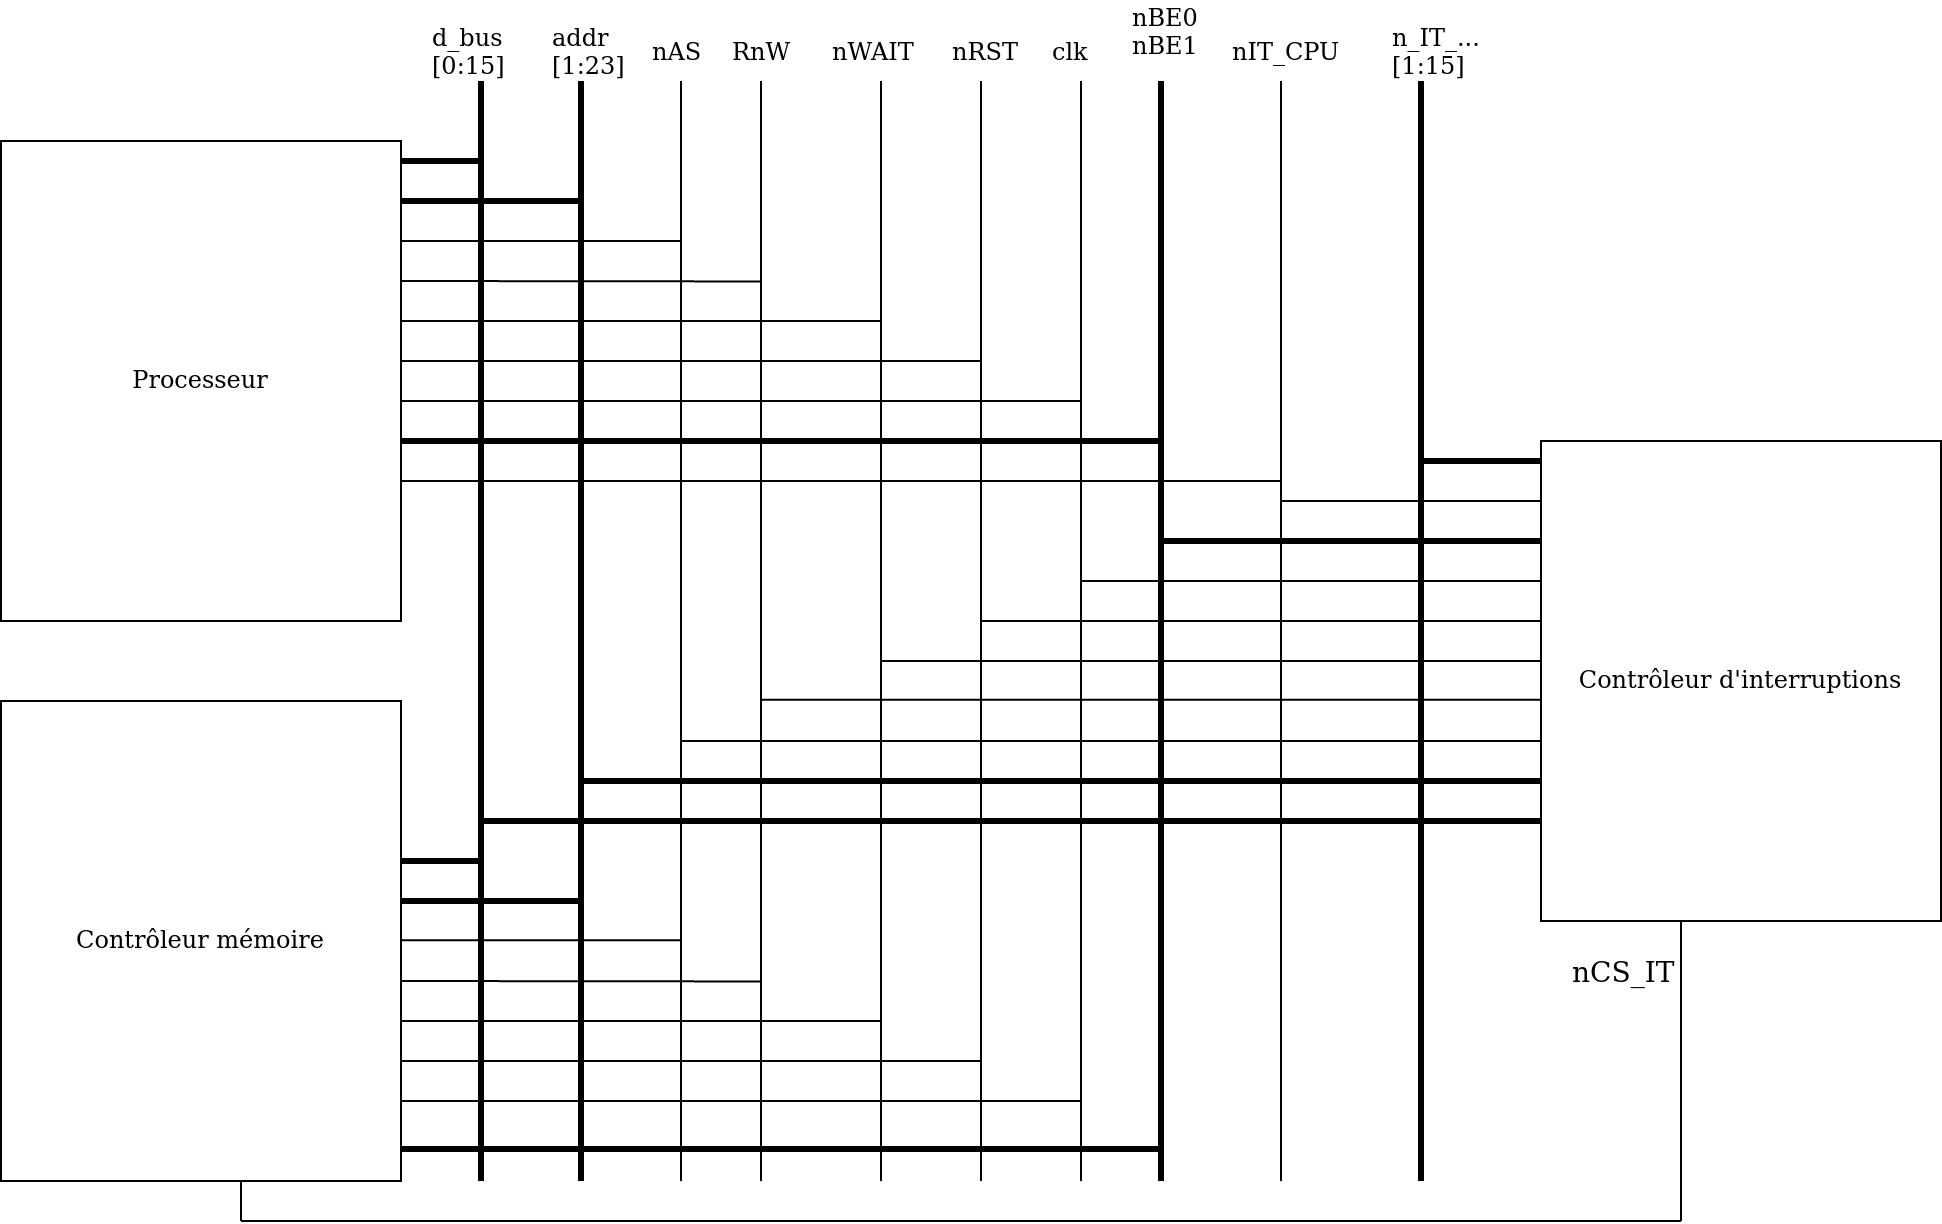
\includegraphics[width=1\linewidth]{figure/schema_cablage.png}
	\caption{Schéma de câblage de l'IP à concevoir, du contrôleur mémoire et du processeur}
	\label{fig:schema_cablage}
\end{figure}
	
Le contrôleur d'interruptions est également câblé avec plusieurs autres IPs du SoC.
Il y a par exemple le processeur avec lequel le signal nIT\_CPU est commun.
D'autre part le contrôleur mémoire est connecté avec le contrôleur d'interruptions par le signal nCS\_IT. L'ensemble des périphériques du SoC peut également envoyer un signal d'interruption représenté par nIT\_ $\dots$\\
	
Le schéma présenté ci-dessus ne précise pas le sens des signaux.
Il n'est donc pas possible de savoir quelles sont les entrées et sorties du contrôleur d'interruptions.
Également, les noms des 4 interruptions externes et des 11 autres provenant de divers périphériques ne sont pas donnés.
La figure et le tableau suivant présentent les entrées et sorties du point de vue de l'IP à concevoir ainsi que le rôle de chaque signaux. 
	
\begin{figure}[H]
	\centering
	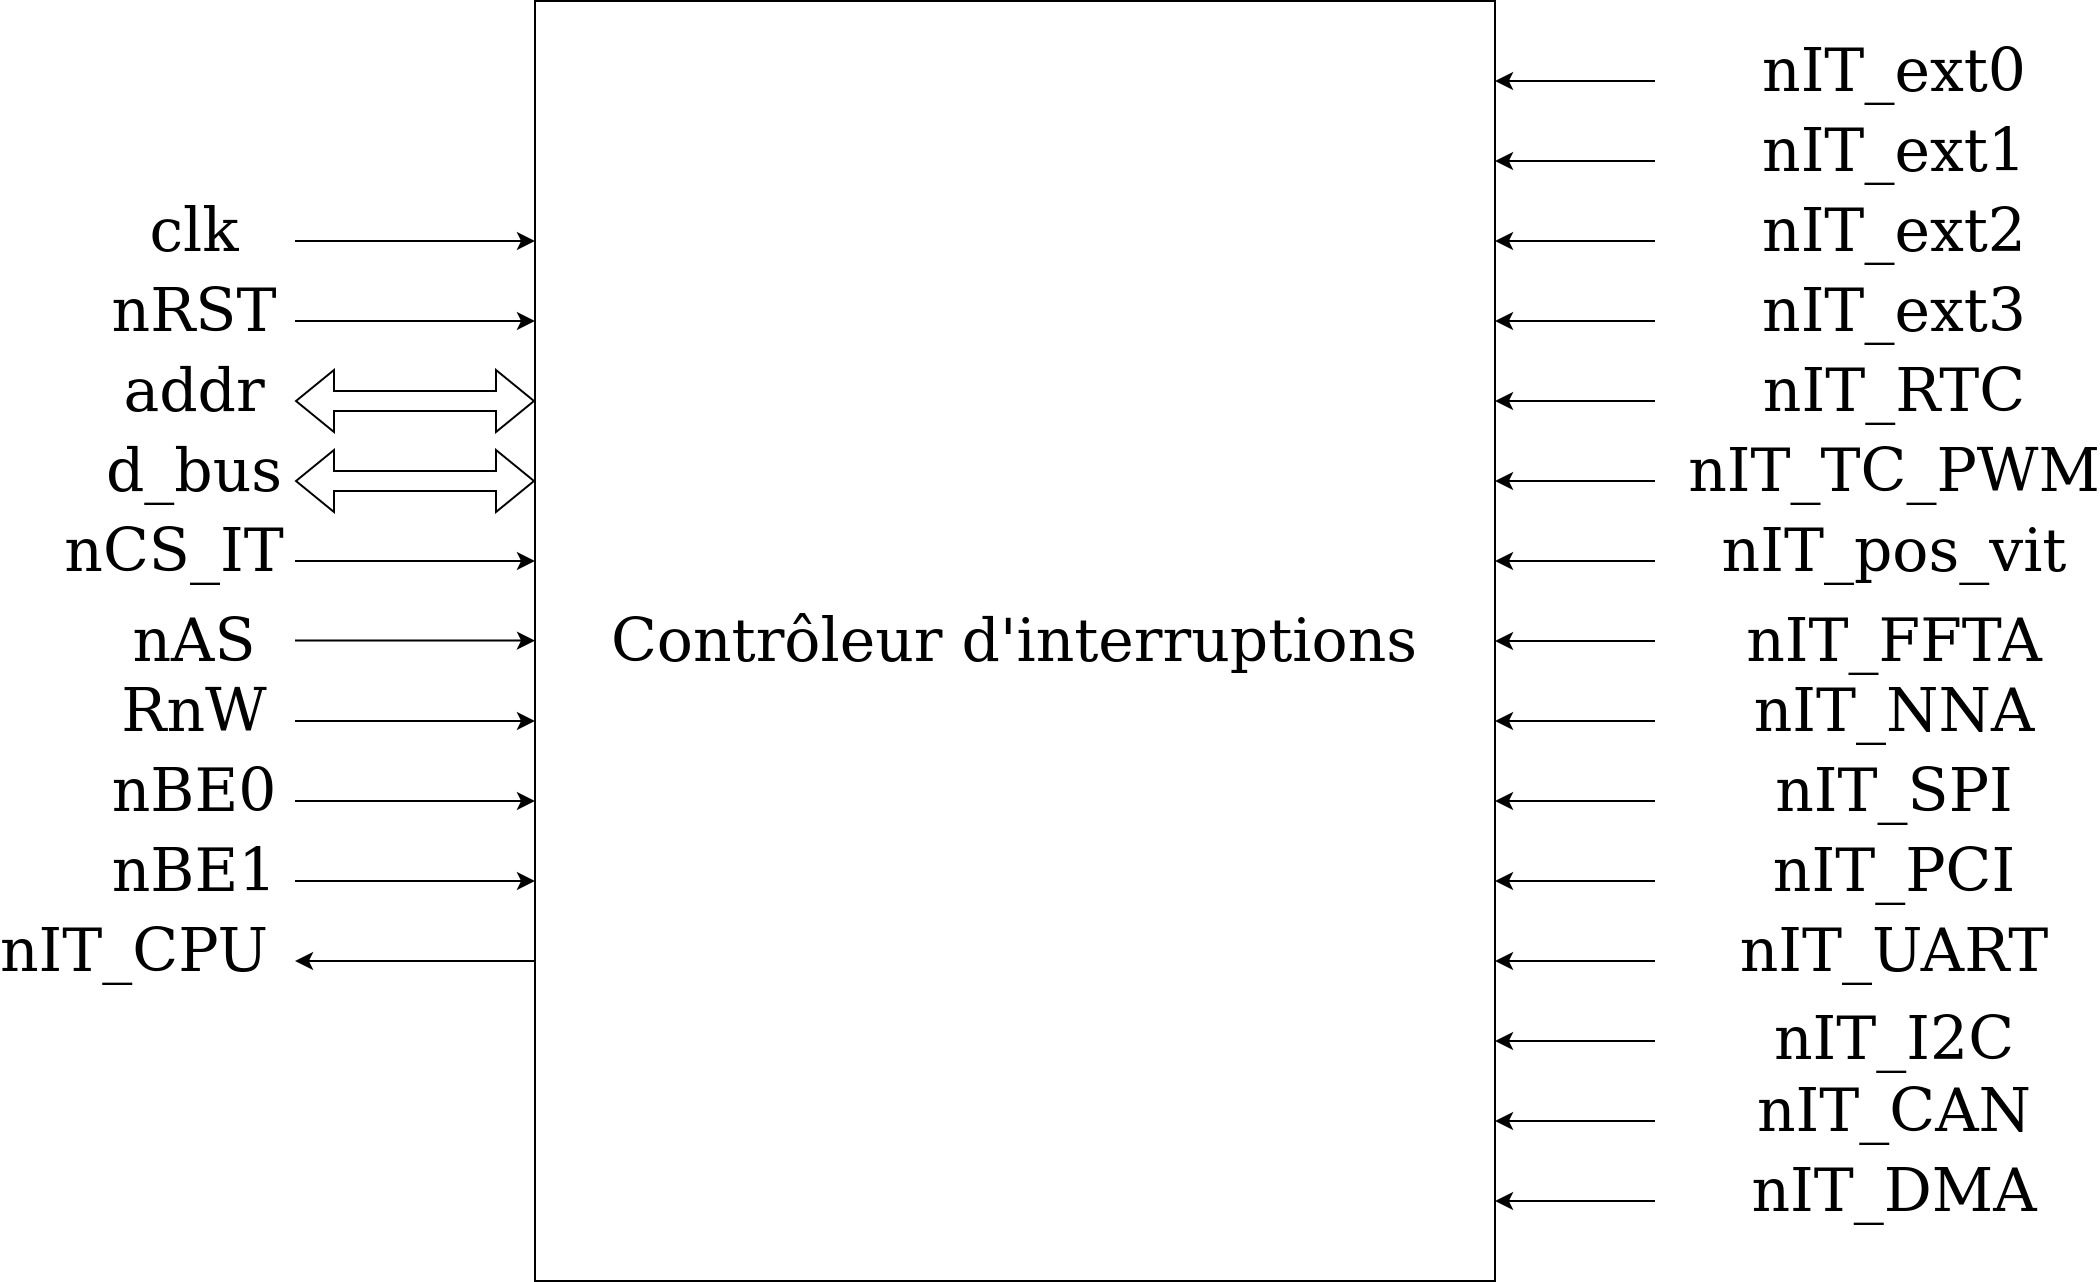
\includegraphics[width=1\linewidth]{figure/delimitation_systeme.png}
	\caption{Entrées et sorties de l'IP à concevoir}
	\label{fig:inout_ip}
\end{figure}


\begin{table}[H]
	\centering
	\begin{tabular}{|c|c|c|}
		\hline
		Nom & Sens & Rôle\\
		\hline
		clk & Entrée & Signal d'horloge\\
		\hline
		nRST & Entrée & Signal de réinitialisation\\
		\hline
		addr & Entrée et sortie & Bus d'adresses\\
		\hline
		d\_bus & Entrée et sortie & Bus de données\\
		\hline
		nCS\_IT & Entrée & Signal de sélection du périphérique en cas \\
		& & d'opérations de lecture ou d'écriture\\
		\hline
		nAS & Entrée & Signal indiquant la présence d'une valeur\\
		& & sur le bus d'adresse\\
		\hline
		& & Signal d'écriture ou de lecture\\
		RnW & Entrée & 0 : écriture\\
		& & 1 : lecture\\
		\hline
		 & & Signal indiquant la structure de la mémoire\\
		nBE0 & Entrée & 0 : little-endian\\
		& & 1 : big-endian\\
		\hline
		& & Signal indiquant la taille de la donnée\\
		nBE1 & Entrée & 0 : 8 bits\\
		 & & 1 : 16 bits\\
		\hline
		 &  & Signal pour le processeur avertissant \\
		nIT\_CPU & Sortie & qu'une interruption est demandée de la part d'un \\
		& & périphérique\\
		\hline
		nIT\_ext0 & Entrée & Signal d'interruption extérieure numéro 0\\
		\hline
		nIT\_ext1 & Entrée & Signal d'interruption extérieure numéro 1\\
		\hline
		nIT\_ext2 & Entrée & Signal d'interruption extérieure numéro 2\\
		\hline
		nIT\_ext3 & Entrée & Signal d'interruption extérieure numéro 3\\
		\hline
		nIT\_RTC & Entrée & Signal d'interruption provenant du périphérique RTC\\
		\hline
		nIT\_TC\_PWM & Entrée & Signal d'interruption provenant du Timer et PWM\\
		\hline
		nIT\_pos\_vit & Entrée & Signal d'interruption provenant du\\
		& & périphérique de mesure position et vitesse\\
		\hline
		nIT\_FFTA & Entrée & Signal d'interruption provenant de \\
		& & l'accélérateur transformée de Fourier discrète\\
		\hline
		nIT\_NNA & Entrée & Signal d'interruption provenant de \\
		& & l'accélérateur réseau de neurones\\
		\hline
		nIT\_SPI & Entrée & Signal d'interruption provenant du \\
		& & périphérique de communication SPI\\
		\hline
		nIT\_PCI & Entrée & Signal d'interruption provenant du \\
		& & périphérique de communication PCI\\
		\hline
		nIT\_UART & Entrée & Signal d'interruption provenant du \\
		& & périphérique de communication UART\\
		\hline
		nIT\_I2C & Entrée & Signal d'interruption provenant du \\
		& & périphérique de communication I2C\\
		\hline
		nIT\_CAN & Entrée & Signal d'interruption provenant du \\
		& & périphérique de communication CAN\\
		\hline
		nIT\_DMA & Entrée & Signal d'interruption provenant du \\
		& & périphérique d'accès direct à la mémoire.\\
		\hline
	\end{tabular}
	\caption{Sens et rôle des signaux}
	\label{tab:sens_role_signaux}
\end{table}
	
Les noms des signaux présentent un suffixe n signifiant que ceux-ci sont actifs à l'état bas.
Par exemple, le signal de sélection nCS\_IT est actif à l'état bas.
Ainsi un signal de sélection à l'état logique 0 signifie que le contrôleur d'interruptions est sélectionné pour une opération de lecture ou d'écriture dans un des registres.


Conventionner ces signaux comme actif à l'état bas n'est pas anodin.
Historiquement, pour des anciennes technologies \gls{TTL}, les signaux actifs à l'état bas sont davantage robustes aux bruits.  
À titre d'exemple, un signal de sélection CS actif à l'état haut sélectionne un périphérique lorsque celui-ci est à l'état logique 1.
Pour des raisons purement physiques (glitch sur le signal, baisse de tension à cause de la résistivité des interconnexions, chute de l'alimentation à cause d'un fort tirage de courant), ce signal à l'état 1 peut passer à l'état de haute impédance Z voir même à l'état bas.
Un tel problème causerait la perdre de données à lire où écrire mais plus généralement des problèmes de sécurité. 


\subsection{Chronogrammes caractéristiques}

\subsection{Contraintes du projet}

La section qui suit traite de la gestion du projet.
Il s'agit de préciser la planification du projet avec des divers livrables à fournir à des dates précises.
La figure (\ref{fig:planning}) ci-dessous est le plan de développement du projet.
Les losanges bleus sont les jalons à fournir.
La conception de cet IP a débuté le 5 octobre 2022 c'est-à-dire à la 40$^{\mbox{ème}}$ semaine de l'année.
Le rendu de l'IP et du rapport de conception s'effectuera la semaine 49.

\begin{figure}[H]
	\centering
	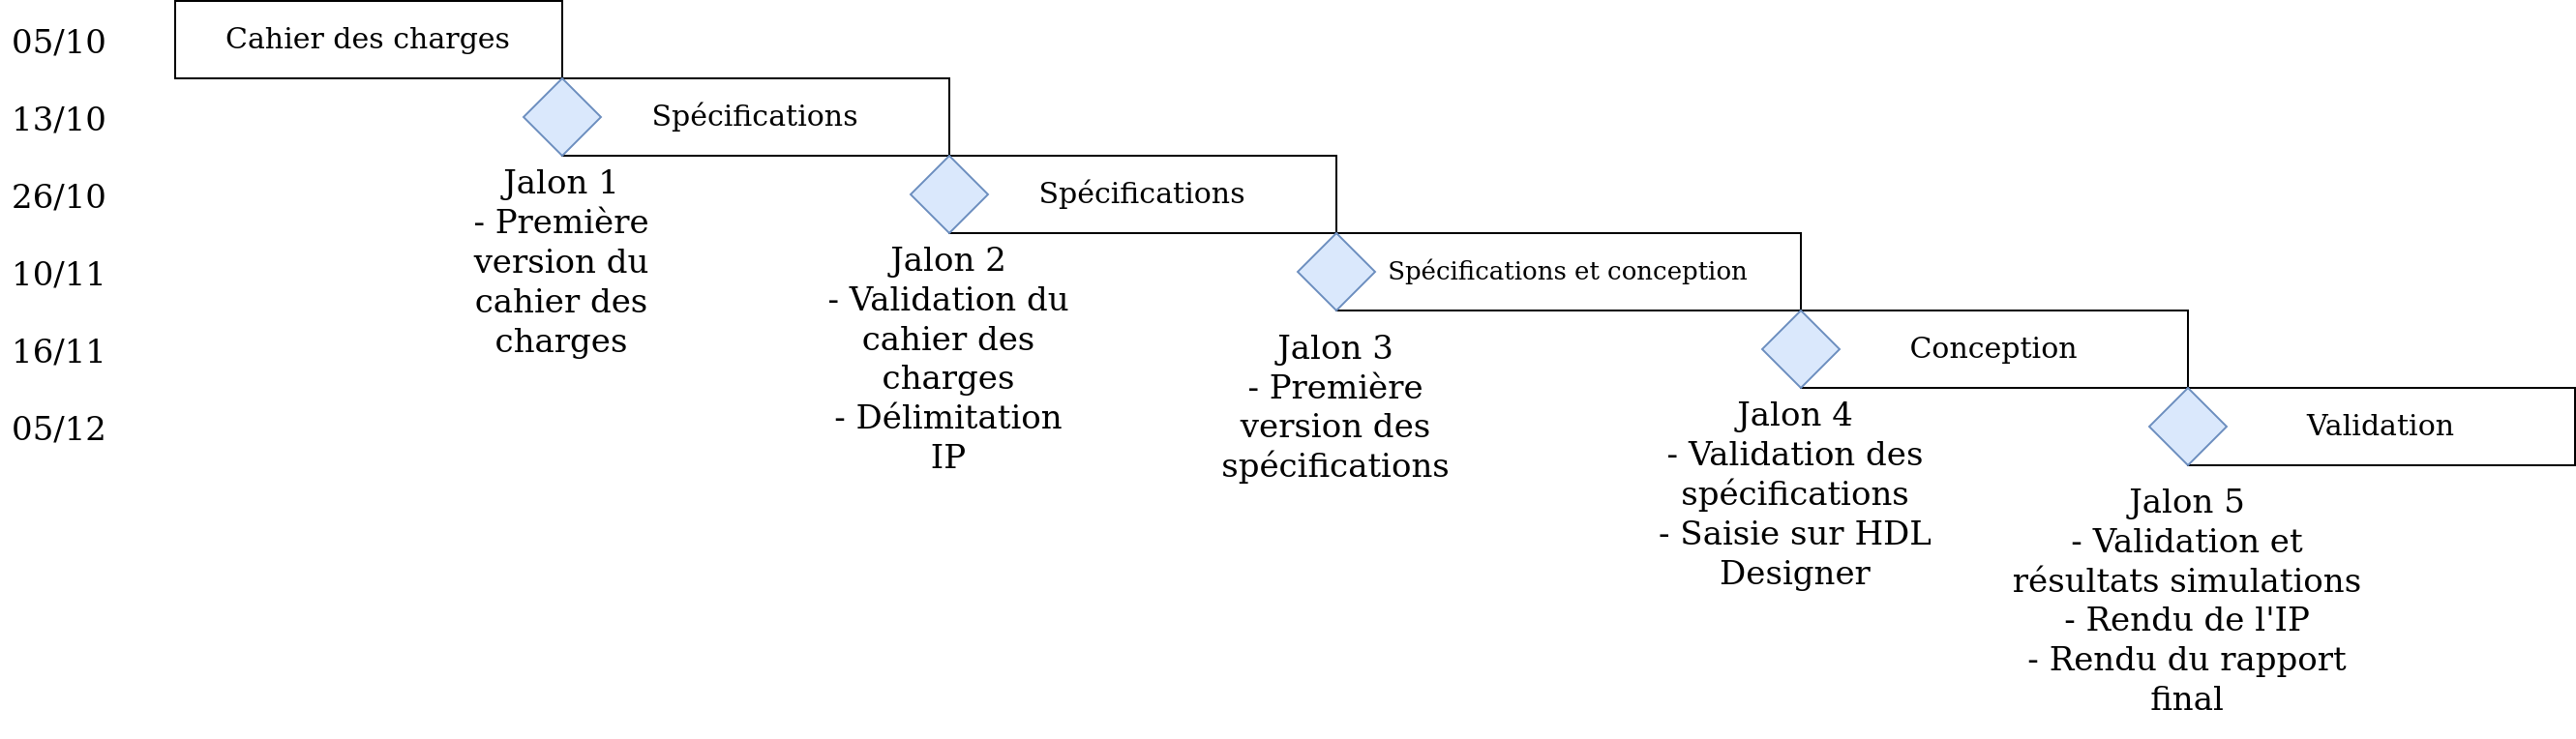
\includegraphics[width=1\linewidth]{figure/planning.png}
	\caption{Planification du projet avec ses jalons}
	\label{fig:planning}
\end{figure}

Également, le projet est contraint d'un point de vue ressources disponibles.
La liste suivante présente les ressources attribuées pour la conception de ce contrôleur d'interruptions.

\begin{itemize}
	\item 2 concepteurs
	\item Outils EDA de Mentor Graphics (propriété de Siemens EDA)
	\item Carte d'évaluation ZYNQ-7 basé sur un FPGA Zynq-7000
\end{itemize}
